\section{Begrenztes Wachstum}
Es gibt Sachverhalte, die erfodern, dass eine e-Funktion/Exponential Funktion nicht in ihrer ursprünglichen Form vorliegt. Dass bedeutet, dass nicht jeder Sachverhalt gleich mit einer Funktion, der Form $f(x)ae^{kx}$ oder $f(x)=a\cdot b^x$ modeliert werden kann. So eignet sich das  Beispiel eines Glasses Milch, der in einen Raum gestellt wird und somit sich Temperatur der auf die Raumtemperatur angleicht. Den Verlauf der Temperatur darzustellen in Abhängikeit der Zeit ergibt nur auf eine Art Sinn.
\begin{figure}[h]
\centering
	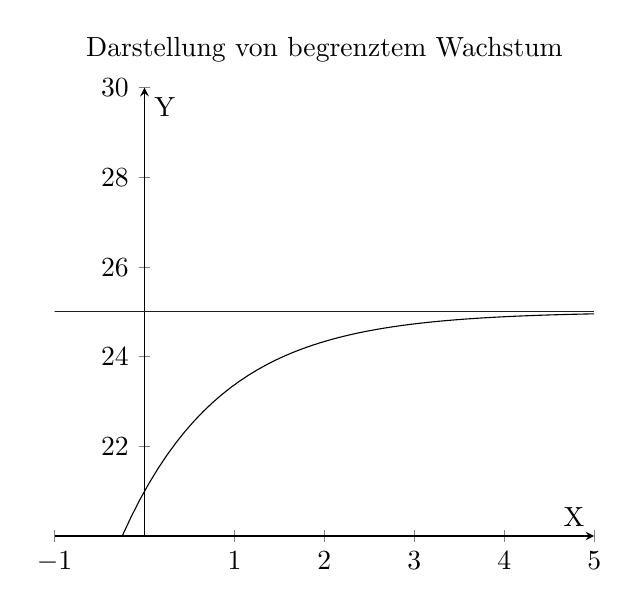
\begin{tikzpicture}
		\begin{axis}[
		title={Darstellung von begrenztem Wachstum},
		axis lines=middle,
		clip=true,
		xlabel={X},
		ylabel={Y},
		xmin=-1,
		xmax=5,
		ymin=20,
		ymax=30
		]
		\addplot[samples=100]{25-4*(exp(-0.9*x))} node[right,pos=1]{$25-4e^{-0.9x}$};
		\addplot[color=blue, samples=100]{25} node[right,pos=1]{$25$};
		\end{axis}
	\end{tikzpicture}
	\caption{Der Graph von $25-4e^{-0.9x}$ konvergiert zu $25$}
\end{figure}
Die 25 Grad stellen das Minimum der Temperatur, welche der Kaffe erreichen kann, dar. Somit kann nur Abb 3 zutreffen auf eine mit einem begrenzten Wachstum. Um nun den Prozess des Modellierens, der Funktion, welche die Temperatur des Kaffes darstellt, fortzuführen, ist es wichtig sich die Informationen, welche gegeben sind, anzuschauen. So kann beispielsweise aus der Information, dass der Kaffe jeden Moment um 9\% wärmer wird, gezogen werden, dass $e^{-0.09}$ die alleinig um die Abnahme, sondern auch um die Begrenzung. Mit logischem Überlegen kann man nun den Graphen im Koordinatensystem verschieben. Dies erfolgt durch das Ändern der Parameter der Normalform. Da die Sättigungsgrenze bekannt ist, können wir mit dem Parameter $e$ den Graphen nach oben schieben, sodass der Graph bereits gegen $25$ konvergiert. Wissen wir nun den Startwert bzw. die Temperatur bei der wir den Kaffee raus gestellt haben, können wir konkret den Bereich der Wertemenge eingrenzen. Nehmen wir an, dass der Kaffe $4\deg$ kalt war, kann man sich nun den Bereich, der für die Rechnung relevant ist, berechnen. Dies wird mit der Hilfe von Subtraktion des Startwertes Minus die Sättigungsgrenze gemacht. Dies ist wichtig, weil wir einen Startwert benötigen für unsere Funktion. Normalerweise kann man einfach $a$ verändern, allerdings bedingt $-25$ diesen Wert. Unser Startwert ist also $25-4$. Daraus folgt, dass die Funktion wie folgt aussehen muss. \[f(x)=-21e^{-0.09x}+25\]
\pagebreak